\documentclass[
10pt, % Main document font size
a4paper, % Paper type, use 'letterpaper' for US Letter paper
oneside, % One page layout (no page indentation)
%twoside, % Two page layout (page indentation for binding and different headers)
headinclude,footinclude, % Extra spacing for the header and footer
%BCOR5mm, % Binding correction
useAMS,
usenatbib
]{template/mn2e}  % old: scrartcl
%\usepackage{myaasmacros}
\usepackage{ulem}
\usepackage{color}
%\usepackage{arsclassica} % Modifies the Classic Thesis package
\usepackage[T1]{fontenc} % Use 8-bit encoding that has 256 glyphs
\usepackage[utf8]{inputenc} % Required for including letters with accents
\usepackage{graphicx} % Required for including images
\graphicspath{{Figures/}} % Set the default folder for images
\usepackage{enumitem} % Required for manipulating the whitespace between and within lists
\usepackage{lipsum} % Used for inserting dummy 'Lorem ipsum' text into the template
\usepackage{subfig} % Required for creating figures with multiple parts (subfigures)
\usepackage{amsmath,amssymb}%,amsthm} % For including math equations, theorems, symbols, etc
\usepackage{varioref} % More descriptive referencing
\usepackage{verbatim}
\usepackage{graphicx}
\usepackage[margin=1in]{geometry}
\usepackage{url}
%For hyperlinks:
\usepackage[pdftex,
	breaklinks,
        colorlinks=true,
        urlcolor=blue,		% \href{...}{...} external (URL)
        filecolor=blue,		% \href{...} local file
        citecolor=blue,		% \href{...} local file
        linkcolor=blue,		% \ref{...} and \pageref{...}
        pdftitle={Multi-scale simulations of the Universe},
        pdfauthor={P. Steger, J. I. Read},
        pdfsubject={ETH Zurich, University of Surrey},
        pdfkeywords={},
        pdfproducer={pdfLaTeX},
        hypertexnames=false,
        pdfpagemode=UseNone,
        bookmarksopen=true]{hyperref}
\newcommand\TODO[1]{\textcolor{red}{TODO: #1}}
% \input{structure.tex} Include the structure.tex file which specified
% the document structure and layout

\hyphenation{Fortran hy-phen-ation}
% Specify custom hyphenation points in words with dashes where you
% would like hyphenation to occur, or alternatively, don't put any
% dashes in a word to stop hyphenation altogether

\title{Fighting Hunger with Big Data} % The article title
\author{P. Steger\textsuperscript{1}, E. Elvestad\textsuperscript{2}, N. Tschurr\textsuperscript{3}}
\date{} % An optional date to appear under the author(s)

\begin{document}
\maketitle

\begin{abstract}
We present an application of Big Data to the measure of correlations between large data sets from various sources. Our aim is to see if there is a correlation between weather shocks and child mortality in Africa. We start by first giving an overview of reasons behind high child mortality, previous research and our contribution. We then go in to explaining our technical solution, describing data preparation, mathematical methods, our system architecture and system behaviour. In section 6 we elaborate on issues faced and some of what we have learned.

We find that (i) for Mali there is a weak, but detectable negative correlation between precipitation (11\%) and child mortality of and a slightly larger negative correlation(19\%) for temperature; (ii) Niger shows a positive correlation for precipitation of 35\% and 11\% for temperature; (iii) Some countries show no significant correlations: Chad has a correlation percentage of 0,5\% and 0.4\% for precipitation and temperature correlations respectively; (iv) Remote areas are more likely to show high correlation. For a remote area in Niger, data shows a 66\% correlation on precipitation and an even higher 85\% for temperature.

\end{abstract}

\begin{keywords} Big Data: MapReduce, Amazon Web Services --
    -- Data: Weather, Child Mortality -- Timeseries
\end{keywords}


\setcounter{tocdepth}{2}

{\let\thefootnote\relax\footnotetext{\textsuperscript{1} \textit{
psteger@phys.ethz.ch
}}}
{\let\thefootnote\relax\footnotetext{\textsuperscript{2} \textit{
endree@student.ethz.ch
}}}
{\let\thefootnote\relax\footnotetext{\textsuperscript{3} \textit{
tschurrn@student.ethz.ch
}}}



\section{Introduction}
According to WHO, 6.3 million children under the age of five died in 2013.Children in sub-Saharan Africa are the most threatened. \footnote{\url{http://www.who.int/mediacentre/factsheets/fs178/en/}} More than half of these deaths could have been prevented as the leading causes are curable diseases and malnutrition. About 45\% of these deaths can be linked to malnutrition alone.  Lowering famine and reducing child mortality is one of WHO major goals, as well as a UN millennium goal.

Famine is caused by scarce supply of nutrition, which in turn is caused by
\begin{itemize}
    \item Missing arable land;
    \item inefficient agriculture;
    \item malnutritious food;
    \item contaminated drinking water.
\end{itemize}

The effects of famine are widespread and beyond the scope of this work. We concentrate on one effect, child mortality. With the help of big-data methods, we want to answer the question whether weather extremes are linked to an increase in child mortality in sub-Saharan Africa.

We try to answer the question whether a correlation between weather and child mortality can only be found in certain countries, e.g. poor countries, countries of a specific climate zone or any of the factors described above. Given these results, we will be able to better understand in which countries efforts needs to be taken in order to better the lives of the inhabitants in these countries.

Our setup shows a new approach to the study of effects of extreme weather on child mortality. First, we study correlations on a large scale with different levels of granularity, area, country and super regional. Earlier research mostly looks at micro level with data gathered from single individuals or households in small areas.

Secondly, we study the correlation between temperature and child mortality separately from the correlation between precipitation and child mortality. Several other studies (referenced below) consider at temperature only or a mix of weather events where different features can not be separated. Furthermore our system architecture makes is easy to add new signals of interest, as new data sets become available.

\section{Contribution \& Related Work}
In order to support the need to investigate the correlation between weather and child mortality, past work is presented that supports the thesis that such a correlation exists and has to be taken into account.

A study performed in Mali (Han 2003)
\footnote{\url{http://faculty.apec.umn.edu/pglewwe/Minnconf/papers_by_presenters_last_name/Han_11.6.14_Child\%20Mortality\%20in\%20Mali_HanFoltz.pdf}} found significant effects of rainfall shocks on child mortality. They also showed that household wealth and proximity to health facilities reduce child mortality. Between 2000 and 2010 Mali's GDP grew, but child mortality increased, according to the authors. They conclude that regions facing an increased number of extreme weather events should invest in better infrastructure and health facilities. Jhin Han and Jeremy Foltz investigated child mortality from 1990 to 2011 combined with weather data from 1980 to 2010. The child mortality was investigated for several smaller regions in Mali where agriculture is of great importance, infrastructure is bad and the people are poor. Their work focuses on long-term weather changes and weather shocks as an effect of the climate change. This sets a baseline to compare to.


Another study performed in Senegal (Pitt 1997)
\footnote{\url{http://www.brown.edu/research/projects/pitt/sites/brown.edu.research.projects.pitt/files/uploads/method7a.pdf}} shows that the weather has an effect on the household income in Senegal, which leads to different planning of parenthood and subsequently child mortality. They point out that the seasonal fluctuations in fertility and mortality are more pronounced in developing countries and especially their rural areas because they are more dependent on the agricultural income. This paper shows again that a correlation between weather and child mortality can be expected in many countries sharing similarities with Mali or Senegal. It also shows how importance of household income and how high the dependency on agriculture are.

The traditional approach of these studies has been to gather data locally through house calls and surveys. This is an especially time-consuming method for gathering data and does not scale for larger areas. Our new system enables us to use available digital data that covers a wide range of countries where the accuracy can be checked against previous local studies.

In conclusion, our approach gives new macro level clues as to the correlation between weather extremes and child mortality as well as a modifiable system able to tackle large amounts of data from several different sources. Our approach complements previous research in the sense that different datasets and methods are being used and that the results can be cross verified. Possibly strengthening the arguments of both humanitarian aid organizations and advocates for measures against climate change.


\section{Data Model}
Our data model is conceptually based on three datasets, CDAPs storage system and Spark Resilient Distributed Datasets (RDDs).

The three original datasets used in our project:
\begin{itemize}
\item The child mortality rates are taken from WHO's data repository, missing values are filled in from UNICEF's and the World Bank's repositories.
  \footnote{\url{http://apps.who.int/gho/data/node.main.ChildMortLevels?lang=en}}
\item The population data from SEDAC
    \footnote{\url{http://sedac.ciesin.columbia.edu/data/collection/gpw-v3}}
\item The weather data from Amazon
    \footnote{\url{https://aws.amazon.com/datasets/2759}}
\end{itemize}

The weather in a densely populated area will have a greater effect on the population as a whole than weather in more sparsely populated areas. It was therefore crucial to find a way to weight the weather stations according to their relative effect on the population before aggregating all measurements for a whole country. By combining the population and weather dataset we get a measure of how important each weather station is. We then combine this knowledge further with our statistics over the child mortality. As a last step we use Big Data techniques to calculate the correlations between the weather and child mortality statistics.

\begin{figure}
    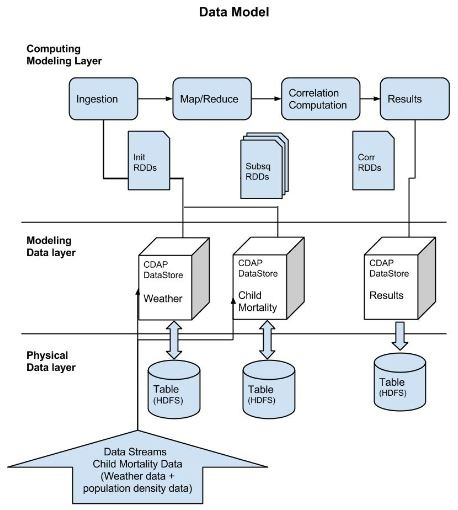
\includegraphics[width=0.5\textwidth]{src/BigChild_DataModel}
    \caption{BigChildren Data Model}
    \label{fig:Data Model}
\end{figure}

These datasets form the foundation of our data model. These are converted to data streams for processing by the CDAP handler. The CDAP handler in turn converts the data into a CDAP data store. The CDAP data store provides an abstraction from the actual representation of where and how the data is stored – be it in HBase, HDFS, or a relational database. In our case, the CDAP data store is physically saved to a HDFS database. CDAP is one of our underlying systems and is explained in depth in section 5 - System architecture.

On initializing the program our stored data is turned into Spark RDDs. During a Map and Reduce phase subsequent RDDs get created to hold intermediate data, as well as reflecting changes to the original RDDs. In the end, a new RDD gets created to hold the results which again is converted to an data store and saved in HDFS for further querying.


\section{Methods}
\subsection{Weather data}
We started by first setting up a small amazon cloud EC2 instance, then adding the snapshot of the weather data. A first comprehension of the data revealed that for each weather station, we were interested in the following properties: country code, latitude, longitude, date, temperature, precipitation.

Data was selected by country, and formatted in the following way:

\begin{itemize}
    \item For each station, the header of the first dataset was copied
    \item All yearly datasets were concatenated
    \item Any whitespaces were reduced to one whitespace only to ease read-in routines
    \item Any missing data were replaced by -1
\end{itemize}


\subsection{Correlation Algorithm}
\label{sec:cor}
Here we explain how we proceed with the precipitation measurements. The temperature is treated analogously.  After reading our data via Flowlets in Spark and preprocessing it to convert to Double’s and SI unit system, we create a first Map function. The key $K$ for this, and some of the following parts, will be the number of the interval the weather measurements were made in, so e.g. for a timestamp of 2010-01-03, and an interval length of 7 days, we get that $K=1$. We subsequently remove any missing measurements (specified by negative entries) by a filter.

\begin{verbatim}
val pdat = wdata
 .map(p => (findInterval((p(2)).toInt,interval),
           (math.floor(p(2)/10000), p(13))))
 .filter( kv => ((kv._2._2) >= 0.0 ))
\end{verbatim}

We want to calculate mean and standard deviation of the precipitation values for interval $K$, given by the collection of measurements in all years for that interval $K$. We can do that only if we have the full distribution of measurements in each interval at our hands, thus we need to collect all entries belonging to the same key first, as is done by groupByKey. We use the cute property that the mean of collections of elements is the same as the mean of all the elements, and calculate the overall standard deviation for efficiency reasons. Both calculations rely on the same collections, thus we only need one groupByKey operation.

\begin{verbatim}
val pred = pdat.map(kv => (kv._1,  kv._2._2))
               .groupByKey()
val pMean=pred.map(kv => (kv._1, mean(kv._2)))
val pSig=pred.map(kv => (kv._1,
  math.max(0.00001, math.sqrt(variance(kv._2)))))
\end{verbatim}

We then run through all values once again to calculate the distance from the mean. This cannot be done in an online algorithm, as the mean is not known a-priori. In a more elegant and marmot-proof way, we would calculate a moving mean, which could be done with one read operation. The degree of outlierness as defined by

\begin{equation*}
d = \frac{\rm{data}(\rm{this year}) - \rm{mean}(\rm{all years})}{\rm{standard\_deviation}(\rm{all years})}
\end{equation*}

is calculated as follows: We join the RDD for precipitation data with the mean value on the interval key $K$, and calculate the absolute distance from the mean in a first step. A second join with the standard deviation allows us to complete the above formula. The measure for outlierness is stored into pOut for later reference.  From now on, we are interested in what year the difference appears in, thus we generate a new key $\tilde{K}=\rm{year}$.

\begin{verbatim}
val pDiff = pdat.join(pMean)
  .map(kv => (kv._1,
              math.abs(kv._2._1._2-kv._2._2)))
val pOut = pDiff.join(pSig)
  .map(kv => (kv._2._1, kv._2._1/kv._2._2))
\end{verbatim}

To compare to the child mortality data, which is given by year and country, we have to look at all time intervals (say, weeks) of a year, and sum up the individual outlier distances.

\begin{verbatim}
val pweather_out = pOut.groupByKey()
                       .map(kv => kv._2.sum)
\end{verbatim}

Thus, we have reduced the full dataset of all precipitation measurements in a year to one single number, that determines how “normal” that year was.

We read in the mortality data, and convert the interesting datafields,

\begin{verbatim}
val mortality: NewHadoopRDD[Array[Byte], String] =
  sc.readFromDataset("childmortality",
    classOf[Array[Byte]], classOf[String])
val mdata = linesDataset.map(kv =>
    parsemVector(kv._2)).cache()
val m_out = mdata.map(p => ((p(0)).toInt, p(4)))
    .map(kv => kv._2)
\end{verbatim}

to calculate the correlation between the time series of weather-extremes and child mortality. We assume a time shift between weather extremes and increase in child mortality that is significantly lower than one year, thus we do not need a full-blown ARIMA analysis, but can as a first approximation work with Pearson correlation measure.

\begin{verbatim}
val pcorr = corr(pweather_out, m_out)
println("pcorr = ", pcorr)
\end{verbatim}

The output is one single number $-1\leq pcorr\leq1$specifying whether there was any
($|pcorr|>0$) correlation, and whether it was a positive or negative
one.

Following modelling decisions were taken in order to achieve higher scalability and performance:

\begin{itemize}
    \item The analysis is done for one single weather station, such that it can be run concurrently for all weather stations;
    \item the data handling was performed as long as possible without grouping or sorting the data, thus any operation beforehand could be kept completely local to a given worker node;
    \item data storage and retrieval is disconnected from analysis, thus no further interaction is necessary
\end{itemize}

\subsection{Geographical distance method}
Here we explain how we proceeded to combine population density data with our weather data.
Both datasets contained geographical coordinates of weather stations and population density centroids respectively. Observe that the combining can be done independent of the rest of the system, and also that the computational complexity whit regard to system as a whole is $O(1)$ sice it only is executed once regardless of system input.

Knowing this we wrote a stand-alone application utilizing the haversine formula. The haversine formula gives the distance between two points on a sphere. Since the earth is not a perfect sphere, a requirement for the haversine function to be completely accurate, it will give a small approximation error. This error is normally found to be less than $0.3$\% depending on latitude and direction of travel.\footnote{http://www.movable-type.co.uk/scripts/latlong.html\#ellipsoid}
For our join we found this to be an acceptable trade off especially since the algorithm is fast, computing $100,000$ iterations in less than a second. A fast computation was of special importance since our two datasets where large and the complexity of the join was $O(N*M)$.

\begin{eqnarray}
 d &=& 2r\arcsin\left(\sqrt{s_\phi + cs_{\phi,\lambda}}\right)\\
 s_\phi &=& \sin^2\left(\frac{\phi_2-\phi_1}{2}\right)\\
 cs_{\phi,\lambda} &=& \cos(\phi_1)\cos(\phi_2)\sin^2\left(\frac{\lambda_2-\lambda_1}{2}\right)
\end{eqnarray}
%\newline
%\noindent
%$d =$
%\newline
%\noindent
%\begingroup
%  \small
%  \thinmuskip=\muexpr\thinmuskip*5/8\relax
%  \medmuskip=\muexpr\medmuskip*5/8\relax
%  $
%    \displaystyle
%2 r \arcsin\left
%(\sqrt{\sin^2\left(\frac{\phi_2 - \phi_1}{2}\right) +
%\cos(\phi_1) \cos(\phi_2)\sin^2\left(\frac{\lambda_2 - \lambda_1}{2}\right)}\right)
%  $%
%\endgroup\\

\begin{itemize}
\item $d$ is the distance between the two points
\item $r$ is the radius of the sphere,
\item $\phi_1, \phi_2 $: latitude of point 1 and latitude of point 2
\item $\lambda_1, \lambda_2$: longitude of point 1 and longitude of point 2
\end{itemize}

For the matching we read in the data from each dataset and for each station compute the haversine distance to a population density centroid. We then keep a record of the smallest distance found. A filter is applyed for removing an entry is the distance is above 100KM. Stations outside this range where shown to be boys in the sea or other remote weather stations having little to no effect on the lives of people, a mach here would give the wrong impression on the stations imprtance. In the end we read out a pairing of the station and its best match in the population density dataset.

\section{System Architecture}
The broad architecture utilizes following abstraction layers:
\begin{itemize}
\item Amazon EC2;
\item the CDAP platform;
\item CDAP app for setup;
\item project code for calculation;
\end{itemize}


\subsection{Comparison with Old Setup}
Our proof of concept architecture utilized the entire technology stack from Hortonworks. For our fully scalable version we have changed to The Cask Data Application Platform (CDAP). CDAP is a layer of software running on top of Hadoop platforms such as the Cloudera Enterprise Data Hub or the Hortonworks Data Platform. It defines and implements a collection of services and a set of SPIs (Service Provider Interfaces) that runs applications on existing Hadoop infrastructure such as HBase, HDFS, YARN, MapReduce, Hive, and Spark.

The benefits that we get from this high level approach over our initial architecture is:
\begin{itemize}
    \item Virtualization of data in the Hadoop environment through logical representations of underlying data
    \item Virtualization of applications through application containers
    \item Services and tools that enable faster application creation in development and higher degrees of operational control in production.
\end{itemize}

\begin{figure}
    \centering
    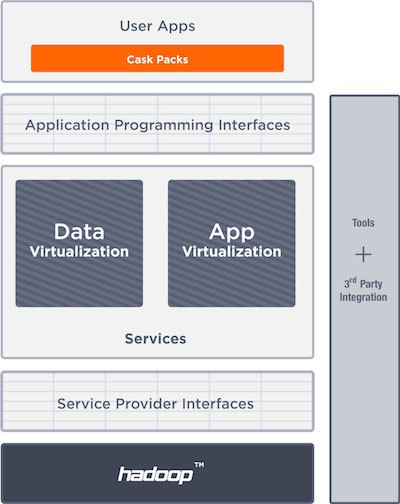
\includegraphics[width=0.95\columnwidth]{src/cdap_architecture}
    \caption{CDAP Functional Architecture}
    \label{fig:cdap}
\end{figure}

As this is our first working example, we have no comparison to an old, unscalable version, and thus cannot tell the influence of our measures for scalability on runtime and space requirements. See the later sections for the single measures found on that code status.


In this section we will further explain Amazon EC2, the CDAP platform and the project code.


\subsection{Architecture and Code}
Amazon Elastic Compute Cloud (Amazon EC2) is a web service from Amazon that provides remote, secure and resizable computing capacity. EC2’s web interface allows to obtain and configure changes in capacity with minimal effort and provides complete control of its computing resources. Amazon EC2 also provides tools to build failure resilient applications and quickly recover from common failure scenarios. Taking advantage of Amazons large scale operations we also reduce the cost of our operation.

\begin{figure}
  \centering
  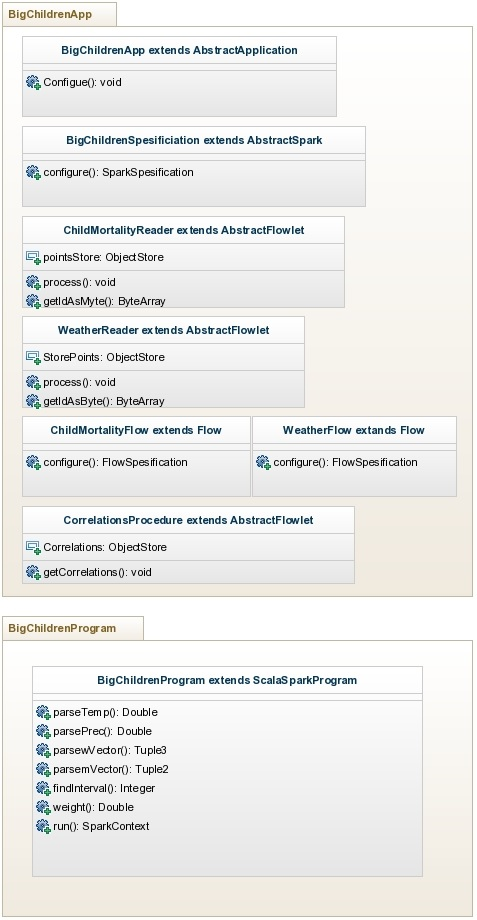
\includegraphics[width=0.50\textwidth]{src/BigChild_ClassDiagram2}
  \caption{Class diagram - CDAP APP}
  \label{fig:classdiagram}
\end{figure}

The Cask Data Application Platform offers benefits across the full range of Hadoop use cases by enabling the reuse of data and applications, and by providing operational controls difficult to implement without virtualization, a secured router, and supporting runtime services. There are two classes of use cases which are both common and critical and where the capabilities of CDAP are uniquely valuable. One specific class of applications are Extract, Transform, and Load (ETL) apps, and another is a more general type which requires a blend of batch and real-time analytics. For our project we have utilized CDAPs solutions to build robust ETL apps.

\footnote{CDAP whitepaper - \url{http://docs.cask.co/collateral/current/cdap-whitepaper-1.0.0.pdf}}


%- http://cask.co/wp-content/uploads/Diag_Architecture.png]
\begin{figure*}
  \centering
  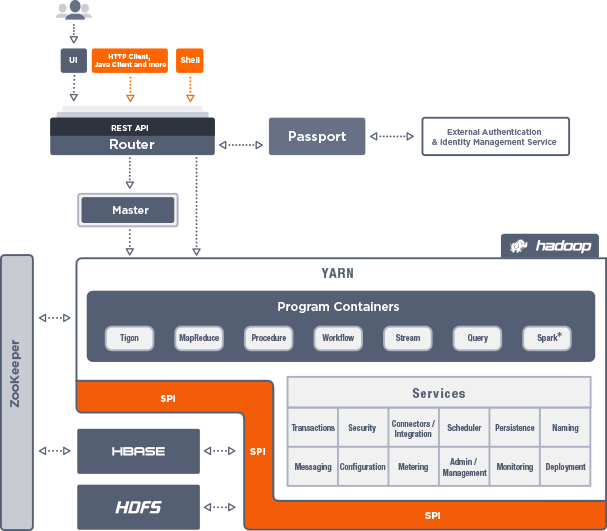
\includegraphics[width=0.95\textwidth]{src/Diag_Architecture}
  \caption{CDAP System Architecture}
  \label{fig:cdapsystem}
\end{figure*}

Our program running in CDAP consists of two main classes. The "BigChildrenApp" class is for configuring the CDAP run-time environment. This includes setup of streams, flows, procedures and output storage. The "BigChildrenProgram" on the other hand is a Scala class implementing the project logic, the actual steps involved in the computation for the correlations. Both classes ties in to the general CDAP environment through inheritance from CDAPs API. Furthermore, the two classes relie on a set of support classes handling the specifics of I/O and computations as shown in the class diagram, \ref{fig:classdiagram}.


\subsection{Scalability, Behavior and Limits} \label{Scalability}
Since the execution time increases linearly with problem size our system is very scalable. Some parts of the computations needed in the beginning have a worse increase in response time, but they can be calculated separately and need only be run once for the whole project:  In order to calculate the population density we have to map every weather station to the closest population density centroid. This algorithm has a performance of $\mathcal O(n*m)$, where $n$ is the number of weather stations(60,000) and $m$ the number of population density measurements(250,000). This algorithm is executed once for all the weather stations, independent of the rest of our implementation making it$\mathcal O(1)$ with regard to the problem the system is set to compute (weather measurements and child mortality). Our implementation computes the correlation of the weather data for every single station with the child mortality of the country in which the station is located. Therefore the execution time of our application is expected to grow linearly with the number of stations we are looking at. When applying more resources, the calculations can be done in parallel for all the weather stations.  The execution for a single weather station consists of several time consuming steps. The most time consuming operation is that we need two reduce phases, by \texttt{groupByKey} as described in \ref{sec:cor}. Since the system architecture is made to work in parallel all the way down to a station level it can in theory finish in the time it takes to do the computations for the station with longest weather measurements in a given country, this number typically around 3 minutes. As this is much shorter than the setup time of a full country's worth of weather data, we decided to circumvent the use of a separate key for the weather station in use and rather batch-process all stations for a given country, and parallelize on countries instead.

\subsection{Possible Improvements}
At the moment we find outlier years by calculating the deviation of a specified interval from the mean of this interval over the whole measurement period. As an example we are looking at intervals with the size of a week. For the first interval, in this case the first week of a year, we calculate the deviation of this week and the mean of all first weeks of all years. By computing the mean over the whole period of time we omit the effects that the global climate change has. It means that year at the very beginning and the very end of the measured time get weighted more at the moment. To prevent this we will calculate the deviation from a moving average. The moving average can be calculated using a regression method.  Another improvement we will implement is the use of the functions \texttt{mean} and \texttt{variance}. We use the implementation provided by breeze \footnote{breeze -  \url{http://www.scalanlp.org/api/breeze/index.html\#breeze.stats.DescriptiveStats\$}}. When looking into the source code of those functions we figured out that they both use the same method but only return a partial result. This means that we iterate twice over our date whereas once would be sufficient.

A further improvement would use the method breeze.stats.meanAndVariance directly, and work with the two outputs, instead of calculating mean and variance independently, thus calling that method twice.
Additionally, de-trending is possible with a moving average.


\section{Main Issues}
\label{sec:issues}
During our work on this project we experienced several small and larger issues. This section first explains some of our challenges before we present our key learnings.

\subsection{Child Mortality}
The dataset contained two different measurements for each datapoint. One containing the probability for a child to die before the age of five and another one denoting the number of children beneath the age of five that die, in relation to a ficticious batch of 1000. The set also contained a comment section switching between standardised error codes, text comments and $None$.  With the use of filtering for different error codes we structured the missing data in a standard $-1$ format. Furthermore, we applied a filtering for retrieving just the deaths per 1000 and for countries in Africa. In the end our child mortality dataset had the form: Indicator, Year, Region, Income group, Country Name, deaths per 1000

\subsection{Spark and CDAP}
Our main issue with the CDAP approach turned out to be the access to the final output: A simple output through a logger is not easily done, as it is unclear what logger CDAP is using internally, and the readily available slf4j logger as shown in the examples did not output to the CDAP console. Another approach was chosen to export the final correlation number to a text file via a classic Java FileWriter, but this one aborted with an exception due to the fact that one cannot access the same file concurrently from all the workers. A makeshift output of an RDD to a file did not complain, but nevertheless did not output a thing.
After a lot of trial and error we managed to export the final result to an independent RDD and store it as a Dataset in CDAP.

\subsection{Amazon}
When setting up Amazon EC we run into several different problems. The biggest one was to install Spark. Hortonworks, on which our initial solution from the last milestone was based on couldn’t been installed. We then tried different approaches to install Spark natively. There the problem was that we first used too small an instance and it always ran out of memory. This caused many exceptions not actually correlated to the memory which made debugging very hard. After successfully installing Spark on a bigger Amazon machine (m3.2xlarge) we had to install CDAP. First we tried to install the newest version 2.5.2. Unfortunately it isn’t possible to start CDAP with this version since some dependencies are configured wrongly. After many attempts to get them right, we took an older version and were able to get it running.

\subsection{Key learnings}
If we were to redo this project we would approach the following in a different way:
Our platform, CDAP, was just a few months old when we chose it as the main platform for our project. CDAP provided new and usefull techniques that fit the challenges we faced for our problem, but its lack of documentation, program examples and its several bugs made our work very difficult. Little did it then help that the community around CDAP were small and almost exclusively consisted of the developers.
Needless to say this provided many a challenge for a group that had limited experience programming large distributed systems. In hindsight we probably should have gone for a standalone Spark implementation, because of its superior documentation and larger community.

On the other hand we are glad we chose to learn Scala instead of going with Python or some other previously known language. For the same reasons as above all the documentation for implementing a Spark program is provided in Scala and we strongly believe it would have taken much longer to develop and test our code had we not been able to utilize the Spark documentation and help from the Scala community.

\section{Results}
\subsection{Mali}
Following (station Nr, precipitation correlation, temperature
correlation, population density) tuples were found for Mali:

\begin{table}
    \caption{Correlations for Mali}
    \begin{tabular}{ l l l l }
        \hline\hline
        Station & $p_{\rm corr}$ & $t_{\rm corr}$ & pop. density\\
        \hline
        612020 & -0.2995 & -0.1924 &  0.322\\
        612230 & -0.2466 & -0.4028 & 90.012\\
        612260 & -0.0067 & -0.2069 & 38.498\\
        612300 & -0.0025 &  0.1250 & 25.203\\
        612330 & -0.2798 &  0.1094 &  7.813\\
        612350 &  0.2841 &  0.2992 & 17.569\\
        612400 & -0.2689 & -0.2636 &  8.867\\
        \hline
        \label{tab:MI}
    \end{tabular}
\end{table}


The reliability of these measures cannot be determined by the classical $p<0.05$ procedure as this only yields reasonable values for more than about 500 data points, which in our case is not possible -- the data only features child mortality data for the last 24 years.

We count any correlations above 40\% as significant, given that around 95\% of completely random 20-vectors show correlations in the range $[-0.4, 0.4]$.
Interestingly, all precipitation correlations are negative, but for
one.

We only take stations which have more than 1 year of consecutive weather data and an assigned population density entry inside 100 km.

Wrapping all together, we smooth out the maximum correlations, giving us a precipitation correlation of -0.118 and a temperature correlation of -0.198.

So there is a very weak, but detectable negative correlation between precipitation and child mortality of 11\%, and a stronger, but still weak negative correlation between temperature and child mortality of 19\%.

These findings are indicative of
\begin{itemize}
\item weather influences really matter. The probability that both of these
  correlations are non-0 and still are consistent with completely
  random vectors is diminished by p(corr1)*p(corr2) where p(corr) is
  the Gaussian probability distribution encountered for random
  vectors, with single 95\% confidence intervals of +/-45\%.
\item more children die (statistically) when there are little weather
  extremes. Weather extremes are measured symmetrically, thus we have
  no way of telling whether this comes from too hot or too cold weeks
  -- and this should not be changed, as otherwise we will average out the
  contributions of positive and negative weeks by summing their
  outliernesses over a whole year.
\item Causal connections cannot be found from correlations alone, so
  further investigation will show whether a a) cooler year or b)
  hotter year with less precipitation helps to reduce child mortality,
  and what measures can be taken to mitigate the effects.
\end{itemize}

\subsection{Niger}
\begin{table}
    \caption{Correlations for Niger}
    \begin{tabular}{ l l l l }
        \hline\hline
        Station & $p_{\rm corr}$ & $t_{\rm corr}$ & pop. density\\
        \hline
        610170 & 0.2591 &  0.5588 &  2.673 \\
        610240 & 0.1424 & -0.1195 &  1.213 \\
        610360 & 0.6648 &  0.8257 & 45.908 \\
        610450 & 0.3025 &  0.5888 &  8.370 \\
        610490 & 0.3299 &  0.5179 &  2.740 \\
        610520 & 0.4023 &  0.2978 &118.643 \\
        610850 & 0.2523 &  0.3637 & 21.680 \\
        610900 & 0.1724 & -0.5602 & 98.532 \\
        \hline
        \label{tab:NR}
    \end{tabular}
\end{table}


This one has a very highly correlated station at 66\% and 85\% at high population densities and for the country as a whole, we have a positive correlation with precipitation of 0.350, and a weaker one for temperature of 0.112, not as strong as in the outskirts. A probable reason for this is that people in more remote parts do have less access to hospitals as the ones in more populated areas do.

\subsection{Chad}
\begin{table}
    \caption{Correlations for Chad}
    \begin{tabular}{ l l l l }
        \hline\hline
        Station & $p_{\rm corr}$ & $t_{\rm corr}$ & pop. density\\
        \hline
        647000 &  0.0351 & -0.5118 & 44.594 \\
        647020 &  0.2910 &  0.1326 & 11.370 \\
        647060 &  0.1581 &  0.5210 & 57.187 \\
        647090 & -0.4473 & -0.4917 & 48.060 \\
        647500 &  0.2697 &  0.3688 & 17.744 \\
        647510 &  0.3155 &  0.2445 &  5.949 \\
        \hline
        \label{tab:CD}
    \end{tabular}
\end{table}


Only some of the stations fulfill our requirements, and hold counter-indicating correlations, thus giving a final outcome of neglectable size, precipitation correlation of -0.005 and temperature correlation of -0.039.


\subsection{Scalability and Performance}
Scalability was proven with Mali's weather stations, and performed on one machine with 8 cores. If analyzing one weather station only, the wall-clock time was 2min 31sec, with peak memory of 556MB.
When analyzing 8 weather stations, we use 17min and 805MB, thus a factor 6.8 in time and factor 1.62 for memory. One would expect a factor of 8 for the maximum of these two fractions for linear scaling. It scales sub-linearly, thus.

A proof-of-concept run with 3 amazon instances for 3 additional countries was performed. The full set of countries could thus be analyzed in parallel, and the analyzed data afterwards collected via a git repository. Most of the effort goes into distributing data and starting CDAP on each machine, even when AMI images are used, as we could not find a possibility to store the running state of CDAP.

The main trade-off in this project is that we restricted ourselves to only a small part of the  weather dataset in order to get a connection with another dataset, the mortality. That connection proved to be paramount to our analysis. An additional dataset was used to determine the weighting factors for each correlation, namely the population density. Incorporating all these datasets, and the computations detailed above enforced a simple program flow -- we could not use the population density before we had the correlations, and thus required a non-concurrent step.

With more time on our hands, we would like to connect the weather stations to climate zones as specified by the Koeppen model, and see whether the correlations depend on that classification -- i.e., if there are mostly positive correlations with precipitation outliers in arid areas.

%\bibliographystyle{mn2e}
%\bibliography{sample.bib}

\end{document}
